%% eval.tex
%% $Id: eval.tex 61 2012-05-03 13:58:03Z bless $

\chapter{Evaluation}
\label{ch:Evaluation}
%% ==============================

In this evaluation section, we explore how well the algorithm performs by looking at the performance and examining the decompositions. Our primary interest lies in two aspects, the size of the factors contributing to the decomposition and the coverage of final states by each factor. Through this analysis, we aim to gauge the algorithm's effectiveness in generating meaningful decompositions. This evaluation is pivotal for understanding the algorithm's capability to produce concise and relevant factors, providing insights into the temporal structure of the give labels. For this purpose, the complete f2f dataset was evaluated, described in Section \ref{ch:prelimiaries:real-world-data} consisting of 62 Temporal graphs with 20 to 56 edges each, ignoring loop edges. In total there are 3321 edges with a combined label length of around 2.3 million giving an average label length of 6993. Please not that the data sets represent people looking at each other, a directed edge from node $u$ to $v$ indicates participant $u$ looks at participant $v$ therefore only one edge label at a given time step $t$ has its value set, $\tau(e)[t] = 1$ for exactly one outgoing edged of $u$. This is also visible in the data as only 13.4\% of values is set over all the labels.

\section{Performance Evaluation}
Although performance was not the main focus of the implementation and evaluation, generating \orDecomp for the complete dataset is reasonable fast with around 3 seconds if using the maximal divisors or the greedy approach. The Fourier-transformation takes a lot of additional time for cleaning multiples of a factor as well as replacing factors with multiple set values with a set of factors with only one set value, causing it to run for 1 minute and 45 seconds. All benchmarks were performed on an AMD Ryzen 5 2600X six core processor (12 threads) with a 3.6 GHz base clock and a 4.2 GHz boost clock speed. For memory, 16GB 3200MHz ram and a Samsung evo ssd was used for persistent storage.

\begin{table}[h]
	\begin{tabular}{l|lll}
		 & MaxDivisors & GreedyShortFactors & FourierTransform  \\
		\hline
		 OR-Decomposition & 3.12 & 3.47 & 105 \\
		 AND-Decomposition & 9.85 & 24.83 & - \\
		 	
	\end{tabular}
	\caption{Decomposition time in seconds [s] for complete dataset}
	\label{tab:eval-performance}
\end{table}

It is to not that the \andDecomp is expected to be slower because of considerably greater amount of zeros in the data set as well as the modification to the cover finding algorithm. While with an \orDecomp, each additional factor can only remove outliers, in an \andDecomp an additional factor can also add new outliers. Because of that, the current outliers of a decomposition must be recalculated considering all factors. The Fourier-transform method again increases the amount of factors per cover, which hurts performance. Also it is not implemented for \andDecomp as it is not considered reasonable, since a human would still need to look at all factors since it is an \andDecomp.

\section{Decomposition Evaluation}
Moving on to the decomposition evaluation, we validate each method separately and then compare them against each other. We also benchmark \andDecomp and \orDecomp.

\subsection{Maximal Divisor Decomposition Evaluation}
To get an insight on how well a particular decomposition method is performing, decompose the whole data-set and then plot each factor of each decomposition by its relative size compared to the original \DFA size and the relative amount of covered values of the \DFA by this factor.

\begin{figure}[h]
	\begin{minipage}[h]{0.49\linewidth}
		\centering
		OR-decomposition
	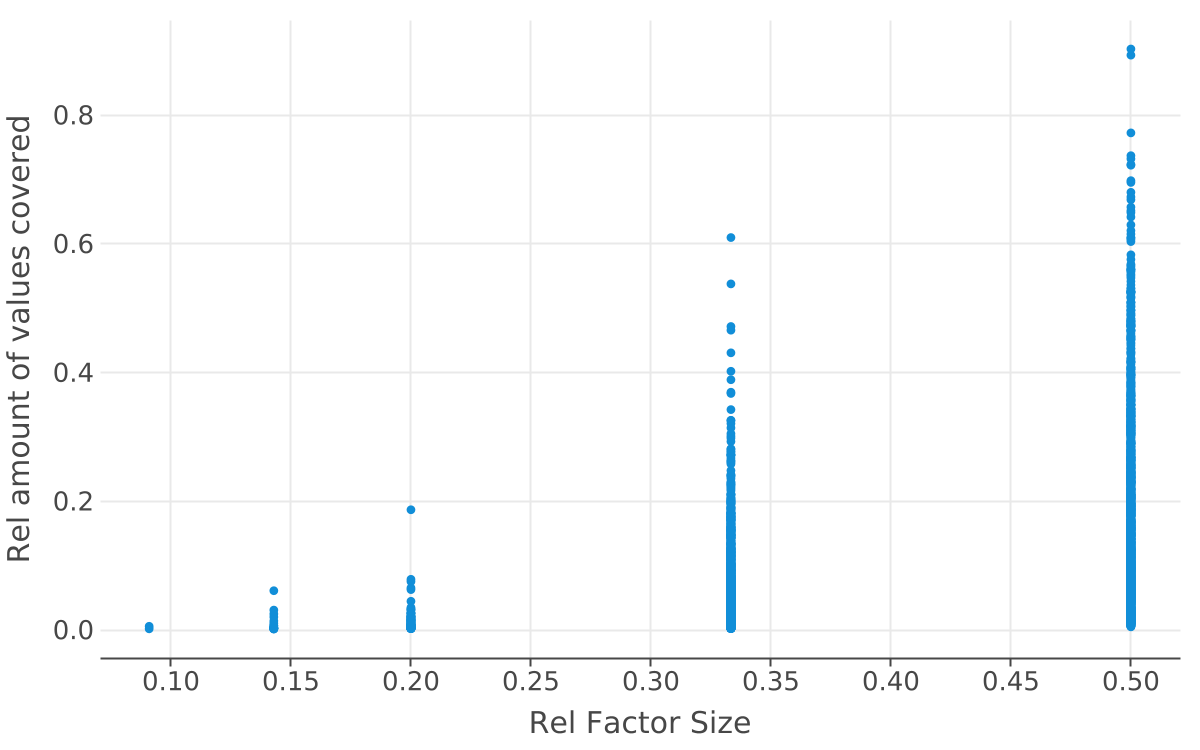
\includegraphics[width=\linewidth]{../plots/point-plots/MAX_DIVISORS-OR-all-relative-values-by-factor-size.png}
	\end{minipage}
	\begin{minipage}[h]{0.49\linewidth}
		\centering
		AND-decomposition
	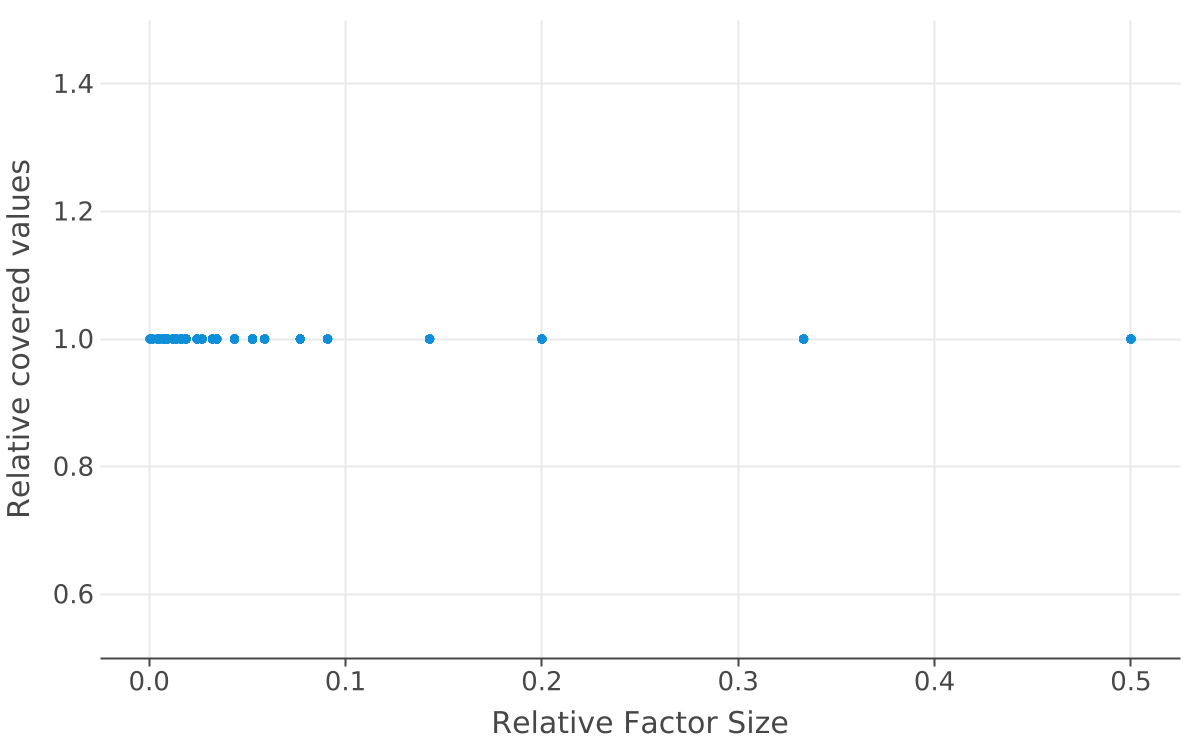
\includegraphics[width=\linewidth]{../plots/point-plots/MAX_DIVISORS-AND-all-relative-values-by-factor-size.png}
\end{minipage}
\label{fig:max-divisor-all-factors}
\caption{Relative amount of covered values by relative factor size}
\end{figure}




\begin{figure}[h]
	\begin{minipage}[h]{0.49\linewidth}
		\centering
		OR-decomposition
		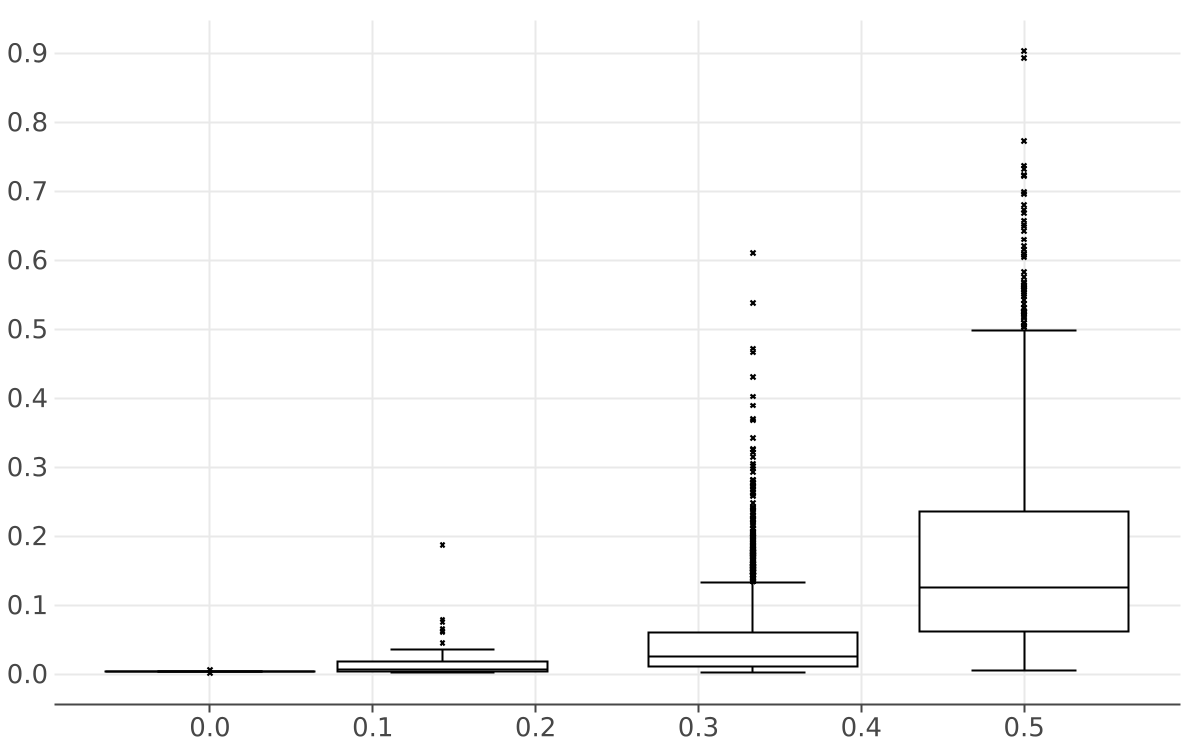
\includegraphics[width=\linewidth]{../plots/box-plots/MAX_DIVISORS-OR-all-relative-values-by-factor-boxplot-dist.png}
	\end{minipage}
	\begin{minipage}[h]{0.49\linewidth}
		\centering
		AND-decomposition
		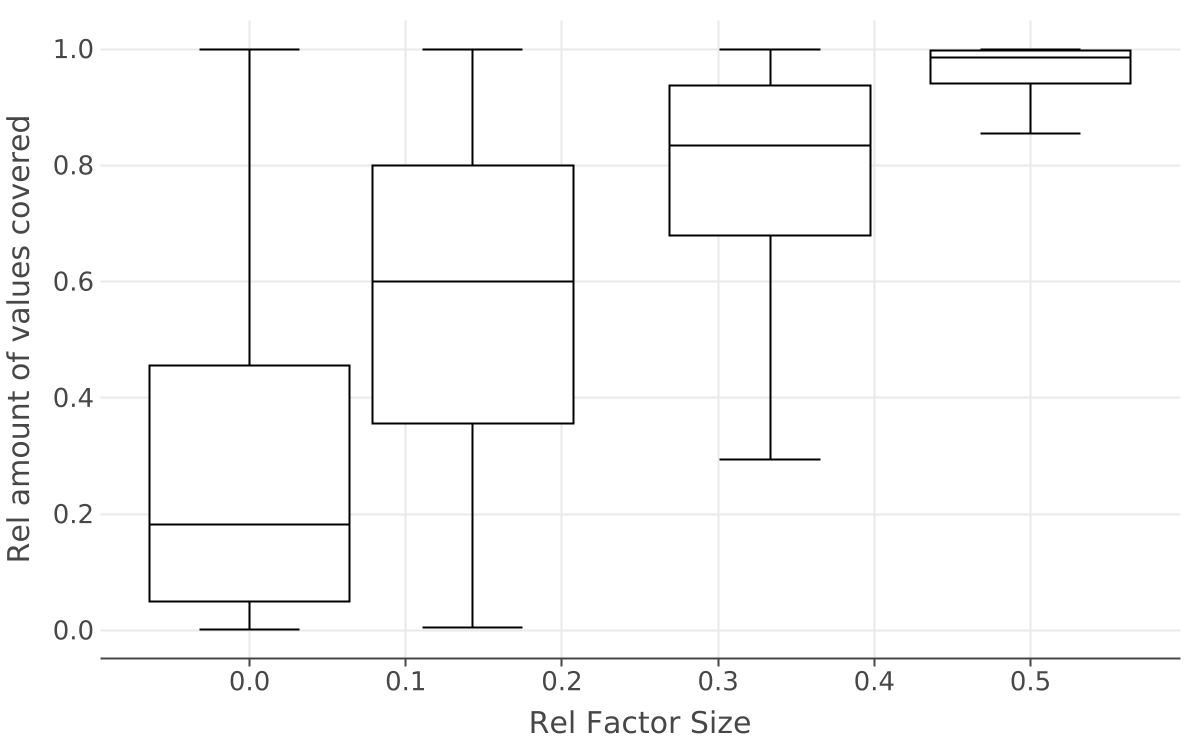
\includegraphics[width=\linewidth]{../plots/box-plots/MAX_DIVISORS-AND-all-relative-values-by-factor-boxplot-dist.png}
	\end{minipage}
	\label{fig:max-divisor-all-factors-box-plot}
	\caption{Relative amount of covered values by relative factor size}
\end{figure}

\subsection{Greedy Short Factor Decomposition Evaluation}

\begin{figure}[h]
	\begin{minipage}[h]{0.49\linewidth}
		\centering
		OR-decomposition
		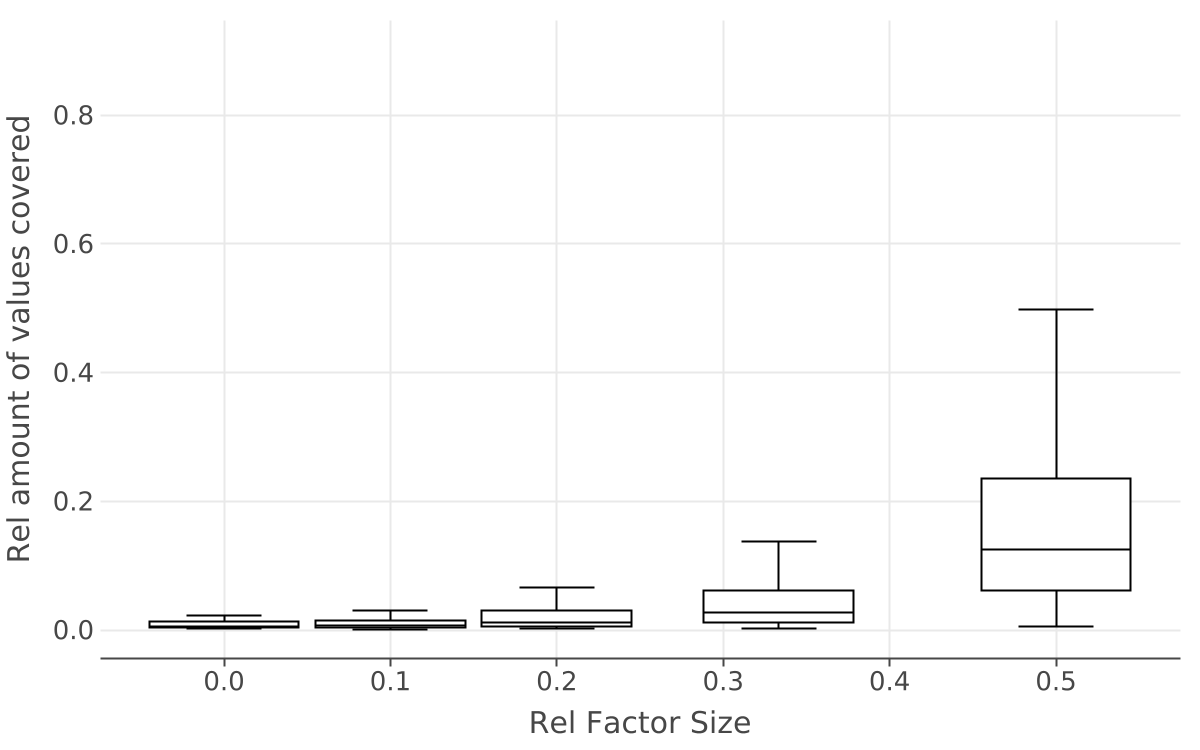
\includegraphics[width=\linewidth]{../plots/box-plots/GREEDY_SHORT_FACTORS-OR-all-relative-values-by-factor-boxplot-dist.png}
	\end{minipage}
	\begin{minipage}[h]{0.49\linewidth}
		\centering
		AND-decomposition
		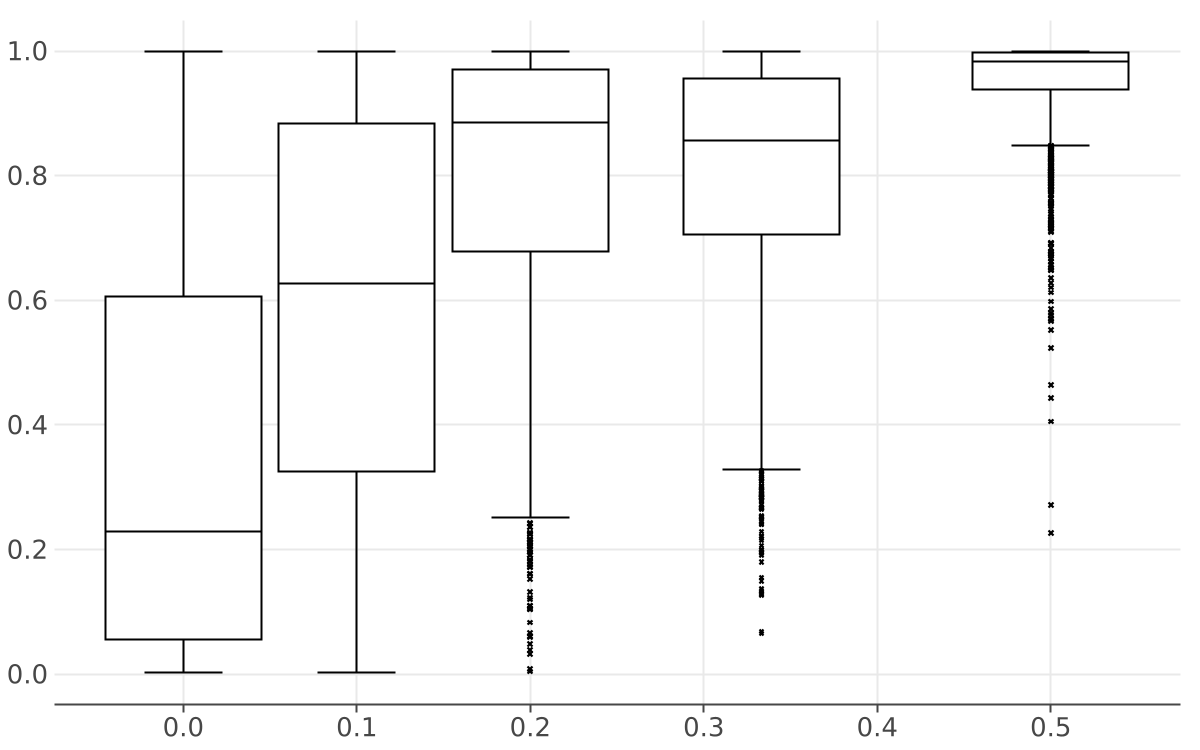
\includegraphics[width=\linewidth]{../plots/box-plots/GREEDY_SHORT_FACTORS-AND-all-relative-values-by-factor-boxplot-dist.png}
	\end{minipage}
	\label{fig:greedy-short-factors-all-factors-box-plot}
	\caption{Relative amount of covered values by relative factor size}
\end{figure}

\subsection{Fourier-Transform Decomposition Evaluation}

\begin{figure}[h]
	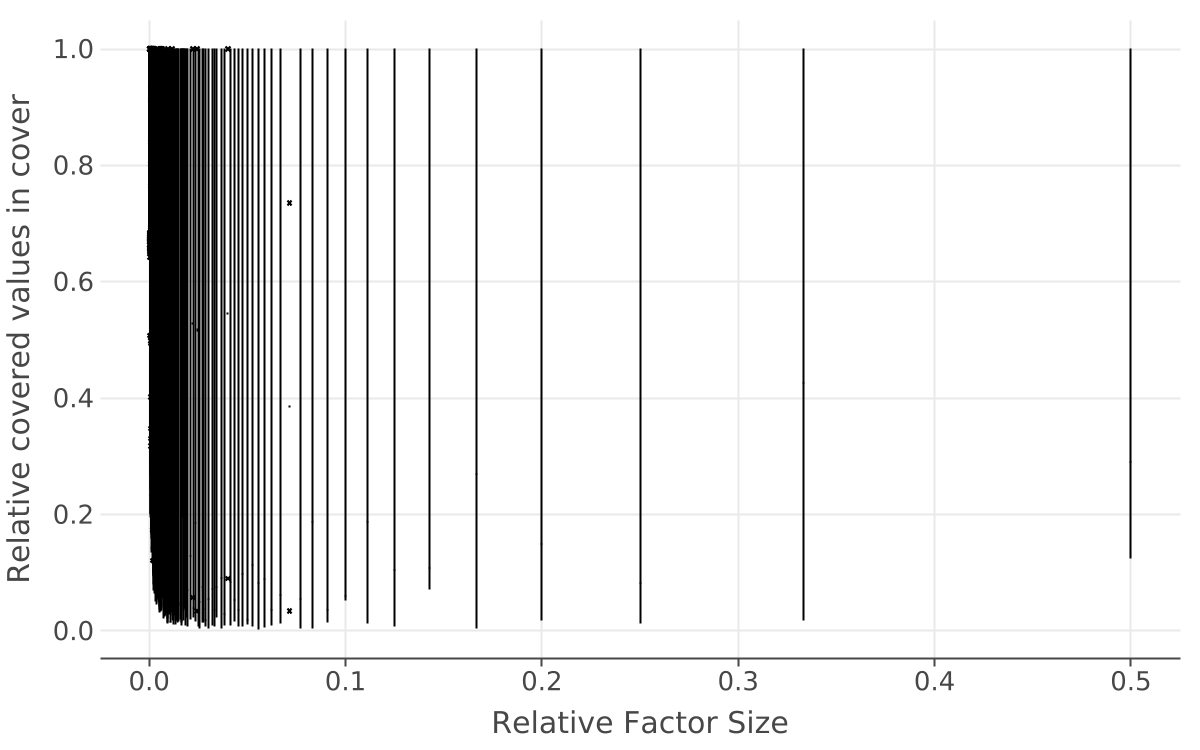
\includegraphics[width=\linewidth]{../plots/box-plots/FOURIER_TRANSFORM-OR-all-relative-values-by-factor-boxplot-outliers.png}
	\label{fig:fourier-all-factors-box-plot}
	\caption{Relative amount of covered values by relative factor size}
\end{figure}

\section{Explainability Evaluation}


%%% Local Variables: 
%%% mode: latex
%%% TeX-master: "thesis"
%%% End: 
